\chapter{Operacje topologiczne na zbiorach}
\label{ch:topog-operacje-zbiorowe}

\noindent\textbf{Cel rozdziału.}
Aksjomaty topologii określają, które podzbiory przestrzeni są otwarte.
Na tej podstawie możemy badać dowolny podzbiór, nawet jeżeli sam nie jest
ani otwarty, ani domknięty. Jego wnętrze opisuje punkty, wokół których
zbiór zawiera całe otwarte otoczenie; domknięcie dodaje punkty, do których
zbiór dochodzi w sensie topologicznym; brzeg odróżnia punkty, w których
każde otoczenie spotyka zarówno zbiór, jak i jego dopełnienie.
Następnie rozróżnimy punkty skupienia i punkty izolowane, wprowadzimy
gęstość i zbiory nigdziegęste oraz pokażemy, że domknięcie można
scharakteryzować bezpośrednio przez cztery aksjomaty Kuratowskiego.
Nie zakładamy metryzowalności, aksjomatu oddzielania $T_1$ ani
niepustości przestrzeni.

W całym rozdziale $(X,\tau)$ oznacza przestrzeń topologiczną, zaś
$A,B\subseteq X$ jej podzbiory. Dopełnienie $A$ w $X$ oznaczamy przez
$X\setminus A$. Otoczenie punktu może nie być otwarte, lecz zgodnie
z definicją zawiera wtedy pewne otwarte otoczenie tego punktu.

\section{Wnętrze i domknięcie}
\label{sec:topog-wnetrze-domkniecie}

\begin{definicja}[Wnętrze i domknięcie zbioru]
\label{def:topog-wnetrze-domkniecie}
Niech $(X,\tau)$ będzie przestrzenią topologiczną i niech $A\subseteq X$.
\emph{Wnętrzem} zbioru $A$ nazywamy zbiór
\[
\operatorname{int}_X A
 =\bigcup\{U\in\tau:U\subseteq A\}.
\]
\emph{Domknięciem} zbioru $A$ nazywamy zbiór
\[
\overline A^{\,X}
 =\bigcap\{F\subseteq X:F\text{ jest domknięty w }X,
                    \ A\subseteq F\}.
\]
Gdy przestrzeń $X$ jest jednoznaczna, piszemy $\operatorname{int}A$
oraz $\overline A$. Rodzina w drugim wzorze jest niepusta,
ponieważ zawiera $X$. Suma zbiorów po prawej stronie pierwszego wzoru
jest określona również dla $A=\varnothing$ i wtedy wynosi $\varnothing$.
\end{definicja}

Intuicyjnie $\operatorname{int}A$ to największy zbiór otwarty
zawarty w $A$, a $\overline A$ to najmniejszy zbiór domknięty
zawierający $A$. Oba określenia wynikają z następującego stwierdzenia.

\begin{stwierdzenie}[Własności ekstremalne]
\label{prop:topog-ekstremalne}
Dla każdej przestrzeni topologicznej $X$ i każdego $A\subseteq X$
zachodzą następujące własności:
\begin{enumerate}[label=(\roman*)]
\item $\operatorname{int}A$ jest otwarty, $\operatorname{int}A\subseteq A$,
      a każdy otwarty $U\subseteq A$ jest zawarty w $\operatorname{int}A$;
\item $\overline A$ jest domknięty, $A\subseteq\overline A$,
      a każdy domknięty $F\supseteq A$ zawiera $\overline A$;
\item $A$ jest otwarty wtedy i tylko wtedy, gdy
      $\operatorname{int}A=A$;
\item $A$ jest domknięty wtedy i tylko wtedy, gdy $\overline A=A$.
\end{enumerate}
\end{stwierdzenie}
\begin{proof}
Wnętrze $A$ jest sumą rodziny zbiorów otwartych,
więc jest otwarte na mocy aksjomatów topologii. Każdy składnik tej
sumy jest zawarty w $A$ i tym samym cała suma jest zawarta w $A$.
Jeżeli $U\subseteq A$ jest otwarty, to jest jednym z sumowanych zbiorów,
zatem $U\subseteq\operatorname{int}A$. Dowodzi to (i).

Domknięcie $A$ jest przecięciem rodziny zbiorów domkniętych,
więc jest domknięte. Ponieważ $A$ jest zawarty w każdym z tych zbiorów,
mamy $A\subseteq\overline A$. Każdy domknięty $F\supseteq A$
występuje w rodzinie przecinanych zbiorów, dlatego
$\overline A\subseteq F$. To dowodzi (ii).

Jeżeli $A$ jest otwarty, to w (i) możemy przyjąć $U=A$,
co razem z $\operatorname{int}A\subseteq A$ daje równość.
Jeżeli $A=\operatorname{int}A$, to $A$ jest otwarty, ponieważ
wnętrze jest otwarte. Analogicznie (ii) dowodzi (iv).
\end{proof}

\begin{twierdzenie}[Charakteryzacja punktowa]
\label{thm:topog-punktowa-charakteryzacja}
Niech $X$ będzie przestrzenią topologiczną, $A\subseteq X$ i $x\in X$.
Wówczas:
\begin{enumerate}[label=(\roman*)]
\item $x\in\operatorname{int}A$ wtedy i tylko wtedy, gdy istnieje
      otwarty zbiór $U$ taki, że $x\in U\subseteq A$;
\item $x\in\overline A$ wtedy i tylko wtedy, gdy dla każdego
      otwartego $U\ni x$ zachodzi $U\cap A\ne\varnothing$.
\end{enumerate}
Oba warunki pozostają równoważne po zastąpieniu otwartych
zbiorów $U\ni x$ dowolnymi otoczeniami punktu $x$.
\end{twierdzenie}
\begin{proof}
Warunek (i) wynika wprost z definicji wnętrza jako sumy
wszystkich otwartych podzbiorów $A$: punkt należy do tej sumy
dokładnie wtedy, gdy należy do przynajmniej jednego jej składnika.

Załóżmy, że $x\notin\overline A$. Zbiór $X\setminus\overline A$
jest wtedy otwartym otoczeniem punktu $x$ i jest rozłączny z $A$,
ponieważ $A\subseteq\overline A$. Zatem warunek (ii) nie zachodzi.
Odwrotnie, niech istnieje otwarty $U\ni x$ rozłączny z $A$.
Wówczas $X\setminus U$ jest domknięty i zawiera $A$,
więc $\overline A\subseteq X\setminus U$. Stąd
$x\notin\overline A$. Otrzymujemy równoważność przez
zanegowanie obu warunków.

Każdy zbiór otwarty zawierający $x$ jest jego otoczeniem.
Jeżeli $N$ jest otoczeniem $x$, to istnieje otwarty
$U$ taki, że $x\in U\subseteq N$.
Dlatego oba kryteria zachowują swoją treść również przy
kwantyfikowaniu po wszystkich otoczeniach.
\end{proof}

\begin{przyklad}[Przedziały w prostej rzeczywistej]
\label{ex:topog-wnetrze-domkniecie-przedzialu}
Rozważmy $\R$ z topologią euklidesową i liczby $a<b$.
Dla $A=[a,b)$ otrzymujemy
$\operatorname{int}A=(a,b)$ oraz $\overline A=[a,b]$.
Rzeczywiście, każdy punkt $x\in(a,b)$ ma przedział
$(x-\varepsilon,x+\varepsilon)\subseteq A$ dla dostatecznie
małego $\varepsilon>0$. Punkt $a$ nie jest wewnętrzny,
bo każde jego otwarte otoczenie zawiera liczby mniejsze od $a$.
Każdy punkt $[a,b]$ należy do $\overline A$: dla $b$
wynika to z faktu, że każde otwarte otoczenie $b$
zawiera liczby z $[a,b)$; dla pozostałych punktów
wynika z zawierania $A\subseteq\overline A$.
Punkt spoza $[a,b]$ ma otwarte otoczenie rozłączne z $A$.

Dla $A=\varnothing$ i $A=\R$ mamy odpowiednio
$\operatorname{int}\varnothing=\overline\varnothing=\varnothing$
oraz $\operatorname{int}\R=\overline\R=\R$.
\end{przyklad}

\begin{twierdzenie}[Rachunek wnętrz i domknięć]
\label{thm:topog-rachunek-wnetrz-domkniec}
Niech $X$ będzie przestrzenią topologiczną, a $A,B\subseteq X$.
Wówczas:
\begin{enumerate}[label=(\roman*)]
\item jeśli $A\subseteq B$, to
      $\operatorname{int}A\subseteq\operatorname{int}B$
      i $\overline A\subseteq\overline B$;
\item $\operatorname{int}(\operatorname{int}A)=\operatorname{int}A$
      i $\overline{\overline A}=\overline A$;
\item $\operatorname{int}(A\cap B)
      =\operatorname{int}A\cap\operatorname{int}B$;
\item $\overline{A\cup B}=\overline A\cup\overline B$;
\item $\operatorname{int}(A\cup B)\supseteq
      \operatorname{int}A\cup\operatorname{int}B$ oraz
      $\overline{A\cap B}\subseteq\overline A\cap\overline B$.
\end{enumerate}
Nie należy w ogólności zastępować obu zawierań w (v)
równościami.
\end{twierdzenie}
\begin{proof}
Jeżeli $A\subseteq B$, to każdy otwarty zbiór zawarty w $A$
jest także zawarty w $B$; po wzięciu ich sum otrzymujemy
pierwsze zawieranie w (i). Z kolei $\overline B$ jest
domknięty i zawiera $A$, więc z minimalności $\overline A$
wynika $\overline A\subseteq\overline B$.

Równości z (ii) wynikają z faktu, że $\operatorname{int}A$
jest otwarty, zaś $\overline A$ domknięty, oraz z (iii)--(iv)
poprzedniego stwierdzenia.

Zbiór $\operatorname{int}A\cap\operatorname{int}B$ jest otwarty
i zawiera się w $A\cap B$, stąd jest zawarty w
$\operatorname{int}(A\cap B)$. W odwrotną stronę,
z monotoniczności i zawierań $A\cap B\subseteq A,B$
wynika $\operatorname{int}(A\cap B)\subseteq
\operatorname{int}A\cap\operatorname{int}B$.

Zbiór $\overline A\cup\overline B$ jest domknięty
jako suma dwóch zbiorów domkniętych i zawiera $A\cup B$.
Stąd $\overline{A\cup B}\subseteq\overline A\cup\overline B$.
Monotoniczność daje oba zawierania
$\overline A,\overline B\subseteq\overline{A\cup B}$,
a zatem również ich sumy. Otrzymujemy (iv).

W (v) zawierania wynikają bezpośrednio z monotoniczności
zastosowanej do $A,B\subseteq A\cup B$ oraz
$A\cap B\subseteq A,B$.
\end{proof}

\begin{przyklad}[Ścisłe zawierania]
\label{ex:topog-scisle-zawierania}
W $\R$ z topologią euklidesową weźmy
$A=[0,1]$ i $B=[1,2]$. Wówczas
$\operatorname{int}A\cup\operatorname{int}B
=(0,1)\cup(1,2)$, podczas gdy
$\operatorname{int}(A\cup B)=(0,2)$.
Punkt $1$ należy tylko do drugiego ze zbiorów.

Dla $A=(0,1)$ i $B=(1,2)$ mamy $A\cap B=\varnothing$,
a więc $\overline{A\cap B}=\varnothing$,
natomiast $\overline A\cap\overline B=\{1\}$.
W ten sposób obie nierówności z poprzedniego
twierdzenia mogą być ścisłe.
\end{przyklad}

\begin{stwierdzenie}[Zależności między dopełnieniem, wnętrzem i domknięciem]
\label{prop:topog-dualnosc-wnetrze-domkniecie}
Niech $X$ będzie przestrzenią topologiczną i $A\subseteq X$.
Wtedy
\[
X\setminus\operatorname{int}A=\overline{X\setminus A},
\qquad
X\setminus\overline A=\operatorname{int}(X\setminus A).
\]
\end{stwierdzenie}
\begin{proof}
Zbiór $X\setminus\operatorname{int}A$ jest domknięty,
gdyż $\operatorname{int}A$ jest otwarty. Zawiera
$X\setminus A$, ponieważ $\operatorname{int}A\subseteq A$.
Dlatego $\overline{X\setminus A}\subseteq
X\setminus\operatorname{int}A$.
Odwrotnie, niech $F$ będzie dowolnym domkniętym
zbiorem zawierającym $X\setminus A$. Wówczas
$X\setminus F$ jest otwarty i zawarty w $A$,
więc $X\setminus F\subseteq\operatorname{int}A$.
Po przejściu do dopełnień otrzymujemy
$X\setminus\operatorname{int}A\subseteq F$.
Przecinając wszystkie takie $F$, dostajemy pierwszą równość.
Druga powstaje z pierwszej po zastąpieniu $A$ przez
$X\setminus A$ i ponownym przejściu do dopełnień.
\end{proof}

\section{Brzeg i zewnętrze zbioru}
\label{sec:topog-brzeg-zewnetrze}

\begin{definicja}[Brzeg i zewnętrze]
\label{def:topog-brzeg-zewnetrze}
Niech $X$ będzie przestrzenią topologiczną i $A\subseteq X$.
\emph{Brzegiem} $A$ nazywamy
$\partial_X A:=\overline A\setminus\operatorname{int}A$,
a \emph{zewnętrzem} $A$ zbiór
$\operatorname{ext}_X A:=\operatorname{int}(X\setminus A)$.
Jeśli przestrzeń jest ustalona, pomijamy indeks $X$.
\end{definicja}

\begin{twierdzenie}[Charakteryzacja brzegu]
\label{thm:topog-charakteryzacja-brzegu}
Niech $X$ będzie przestrzenią topologiczną,
$A\subseteq X$ i $x\in X$. Wówczas:
\begin{enumerate}[label=(\roman*)]
\item $\partial A=\overline A\cap\overline{X\setminus A}$;
\item $x\in\partial A$ wtedy i tylko wtedy, gdy każde
      otwarte otoczenie $U$ punktu $x$ spełnia jednocześnie
      $U\cap A\ne\varnothing$ i
      $U\cap(X\setminus A)\ne\varnothing$;
\item $\partial A$ jest domknięty i
      $\partial A=\partial(X\setminus A)$;
\item $X$ jest sumą rozłączną trzech zbiorów
      $\operatorname{int}A$, $\partial A$ i
      $\operatorname{ext}A$;
\item $\overline A=\operatorname{int}A\cup\partial A$.
\end{enumerate}
\end{twierdzenie}
\begin{proof}
Z twierdzenia o zależności domknięcia i wnętrza od dopełnienia
wynika $X\setminus\operatorname{int}A=\overline{X\setminus A}$.
Dlatego $\partial A=\overline A\cap(X\setminus\operatorname{int}A)
=\overline A\cap\overline{X\setminus A}$, co daje (i).
Równoważność z (ii) wynika z zastosowania punktowej
charakteryzacji domknięcia do $A$ oraz do $X\setminus A$.

W (iii) domkniętość brzegu wynika z (i), bo jest on
przecięciem dwóch zbiorów domkniętych.
Ten sam wzór jest symetryczny względem $A$ i jego
dopełnienia, stąd $\partial A=\partial(X\setminus A)$.

Zbiory $\operatorname{int}A$ i $\operatorname{ext}A$
są rozłączne, bo należą odpowiednio do $A$ i do jego dopełnienia.
Ponadto $\partial A$ nie spotyka żadnego z nich:
z definicji jest rozłączny z $\operatorname{int}A$,
a z (i) i równości
$\operatorname{ext}A=X\setminus\overline A$
wynika rozłączność z $\operatorname{ext}A$.
Niech $x\in X$ nie należy ani do $\operatorname{int}A$,
ani do $\operatorname{ext}A$. Drugi warunek daje
$x\in\overline A$, a pierwszy wtedy $x\in\partial A$.
Dowodzi to (iv). Ponieważ $\operatorname{int}A\subseteq\overline A$,
rozłączna dekompozycja $\overline A$ na
$\operatorname{int}A$ i $\overline A\setminus\operatorname{int}A$
daje (v).
\end{proof}

\begin{przyklad}[Brzeg przedziału i zbioru liczb wymiernych]
\label{ex:topog-brzeg-przyklady}
W $\R$ z topologią euklidesową dla $A=(a,b)$, gdzie $a<b$,
mamy $\operatorname{int}A=(a,b)$, $\overline A=[a,b]$,
$\partial A=\{a,b\}$ i
$\operatorname{ext}A=(-\infty,a)\cup(b,\infty)$.

Dla $A=\Q$ każdy niepusty przedział otwarty zawiera
liczbę wymierną i niewymierną. Zatem
$\overline\Q=\overline{\R\setminus\Q}=\R$, więc
$\partial\Q=\R$. Zarazem $\operatorname{int}\Q=\varnothing$
i $\operatorname{ext}\Q=\varnothing$.
Z tych samych powodów brzeg zbioru liczb niewymiernych
jest całą prostą rzeczywistą.
\end{przyklad}

\begin{figure}[ht]
\centering
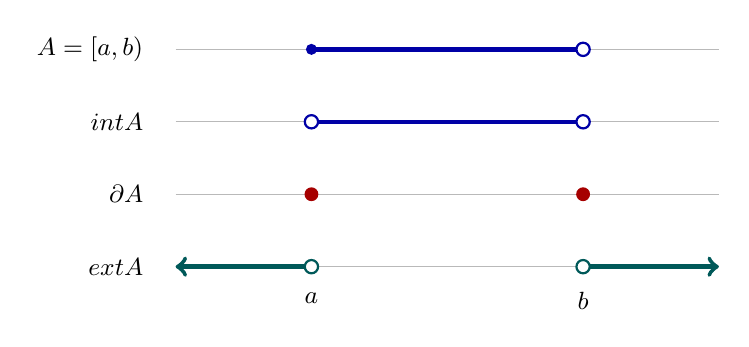
\begin{tikzpicture}[x=1.15cm,y=.92cm, font=\small]
\foreach \y in {0,1,2,3} {
  \draw[gray!55] (-3,\y)--(3,\y);
}
\node[left] at (-3.25,3) {$A=[a,b)$};
\node[left] at (-3.25,2) {$\operatorname{int}A$};
\node[left] at (-3.25,1) {$\partial A$};
\node[left] at (-3.25,0) {$\operatorname{ext}A$};
\draw[blue!65!black,ultra thick] (-1.5,3)--(1.5,3);
\fill[blue!65!black] (-1.5,3) circle (2pt);
\draw[blue!65!black,fill=white,thick] (1.5,3) circle (2.4pt);
\draw[blue!65!black,ultra thick] (-1.5,2)--(1.5,2);
\draw[blue!65!black,fill=white,thick] (-1.5,2) circle (2.4pt);
\draw[blue!65!black,fill=white,thick] (1.5,2) circle (2.4pt);
\fill[red!65!black] (-1.5,1) circle (2.5pt);
\fill[red!65!black] (1.5,1) circle (2.5pt);
\draw[teal!70!black,ultra thick,<-] (-3,0)--(-1.5,0);
\draw[teal!70!black,ultra thick,->] (1.5,0)--(3,0);
\draw[teal!70!black,fill=white,thick] (-1.5,0) circle (2.4pt);
\draw[teal!70!black,fill=white,thick] (1.5,0) circle (2.4pt);
\node[below] at (-1.5,-.22) {$a$};
\node[below] at (1.5,-.22) {$b$};
\end{tikzpicture}
\caption{Wnętrze, brzeg i zewnętrze przedziału $A=[a,b)$
na prostej rzeczywistej. Przy końcach przedziałów pełna
kropka oznacza przynależność do zbioru w danym wierszu.}
\label{fig:topog-rozklad-przedzialu}
\end{figure}

\begin{przyklad}[Brzeg w przestrzeni Sierpińskiego]
\label{ex:topog-brzeg-sierpinski}
Niech $X=\{0,1\}$ i
$\tau=\{\varnothing,\{1\},X\}$. Dla $A=\{1\}$ mamy
$\operatorname{int}A=\{1\}$ oraz $\overline A=X$,
ponieważ jedynym domkniętym zbiorem zawierającym $1$ jest $X$.
Wobec tego $\partial A=\{0\}$.
Dla $B=\{0\}$ zachodzi $\operatorname{int}B=\varnothing$
i $\overline B=\{0\}$, więc również $\partial B=\{0\}$.
Pokazuje to, że brzeg nie musi być zawarty w samym zbiorze:
w tym przypadku $\partial\{1\}$ jest od niego rozłączny,
chociaż zawsze leży w jego domknięciu.
\end{przyklad}

\begin{stwierdzenie}[Brzeg sumy zbiorów]
\label{prop:topog-brzeg-sumy}
Dla dowolnej przestrzeni topologicznej $X$ i dowolnych
$A,B\subseteq X$ zachodzi
$\partial(A\cup B)\subseteq\partial A\cup\partial B$.
\end{stwierdzenie}
\begin{proof}
Niech $x\notin\partial A\cup\partial B$.
Z rozłącznego podziału przestrzeni wynika, że
$x$ należy do wnętrza albo do zewnętrza każdego ze zbiorów
$A$ i $B$. Jeżeli należy do wnętrza przynajmniej jednego
z nich, to należy do $\operatorname{int}(A\cup B)$,
a więc nie leży na brzegu sumy. Jeśli zaś należy do obu
zewnętrz, to otwarty zbiór
$\operatorname{ext}A\cap\operatorname{ext}B$
jest otoczeniem $x$ rozłącznym z $A\cup B$.
Stąd $x\in\operatorname{ext}(A\cup B)$ i znów
$x\notin\partial(A\cup B)$. Dowiedliśmy żądanego zawierania.
\end{proof}

\section{Punkty skupienia i punkty izolowane}
\label{sec:topog-punkty-skupienia}

\begin{definicja}[Zbiór pochodny i punkt izolowany]
\label{def:topog-zbior-pochodny}
Niech $X$ będzie przestrzenią topologiczną i $A\subseteq X$.
Punkt $x\in X$ nazywamy \emph{punktem skupienia} zbioru $A$,
jeżeli każde otwarte otoczenie $U\ni x$ zawiera punkt
zbioru $A$ różny od $x$, czyli
$U\cap(A\setminus\{x\})\ne\varnothing$.
Zbiór wszystkich punktów skupienia $A$ oznaczamy przez
$A'$ i nazywamy \emph{zbiorem pochodnym} zbioru $A$.

Punkt $x\in A$ nazywamy \emph{punktem izolowanym} w $A$,
jeżeli istnieje otwarty $U\ni x$ taki, że
$U\cap A=\{x\}$. Zbiór punktów izolowanych $A$
oznaczamy przez $\operatorname{Iso}(A)$.
\end{definicja}

Punkt skupienia nie musi należeć do samego zbioru $A$.
Z kolei punkt izolowany musi należeć do $A$ z definicji.
Pojęcie punktu skupienia wymaga wyraźnego wyłączenia
samego punktu $x$ z przecięcia: w przeciwnym razie
otrzymalibyśmy charakteryzację domknięcia, a nie zbioru pochodnego.

\begin{twierdzenie}[Domknięcie i zbiór pochodny]
\label{thm:topog-domkniecie-pochodny}
Dla dowolnej przestrzeni topologicznej $X$ i dowolnego $A\subseteq X$
zachodzą równości
\[
\overline A=A\cup A',\qquad
\operatorname{Iso}(A)=A\setminus A'.
\]
\end{twierdzenie}
\begin{proof}
Każdy $x\in A$ należy do $\overline A$.
Jeżeli $x\in A'$, to każde otwarte otoczenie $x$
spotyka $A\setminus\{x\}$, a zatem także $A$;
z charakteryzacji punktowej wynika $x\in\overline A$.
Stąd $A\cup A'\subseteq\overline A$.

Odwrotnie, niech $x\in\overline A\setminus A$.
Każde otwarte otoczenie $x$ spotyka $A$, a ponieważ
$x\notin A$, jego przecięcie z $A\setminus\{x\}=A$
jest niepuste. Zatem $x\in A'$, skąd pierwsza równość.

Dla $x\in A$ równość
$U\cap(A\setminus\{x\})=\varnothing$
jest równoważna warunkowi $U\cap A=\{x\}$.
Punkt $x\in A$ nie jest więc punktem skupienia dokładnie
wtedy, gdy jest izolowany w $A$. Daje to drugą równość.
\end{proof}

\begin{przyklad}[Zbiór wyrazów ciągu i jego punkt skupienia]
\label{ex:topog-pochodny-ciag}
W $\R$ z topologią euklidesową niech
$A=\{1/n:n\in\mathbb N,\ n\ge1\}$.
Każdy otwarty przedział wokół $0$ zawiera $1/n$
dla dostatecznie dużych $n$, więc $0\in A'$.
Dla ustalonego $n$ punkt $1/n$ jest izolowany w $A$:
można wybrać dostatecznie mały przedział wokół $1/n$
niezawierający żadnego innego elementu $A$
(dla $n=1$ wybieramy przedział niewchodzący w $1/2$,
a dla $n\ge2$ korzystamy z luk między kolejnymi wyrazami).
Każdy $x\notin A\cup\{0\}$ ma otwarty przedział
rozłączny z $A$; dla $x<0$ lub $x>1$ jest to oczywiste,
a dla $x\in(0,1)\setminus A$ wynika z istnienia dwóch
kolejnych wyrazów $1/(n+1)<x<1/n$.
Stąd $A'=\{0\}$ oraz $\overline A=A\cup\{0\}$.
\end{przyklad}

\begin{stwierdzenie}[Monotoniczność zbioru pochodnego]
\label{prop:topog-pochodny-monotoniczny}
Niech $X$ będzie przestrzenią topologiczną oraz $A,B\subseteq X$.
Jeśli $A\subseteq B$, to $A'\subseteq B'$.
Ponadto $(A\cup B)'=A'\cup B'$.
\end{stwierdzenie}
\begin{proof}
Jeżeli $x\in A'$, każde jego otwarte otoczenie spotyka
$A\setminus\{x\}\subseteq B\setminus\{x\}$,
więc $x\in B'$. To daje monotoniczność i zawieranie
$A'\cup B'\subseteq(A\cup B)'$.

Jeżeli $x\notin A'\cup B'$, to istnieją otwarte otoczenia
$U\ni x$ oraz $V\ni x$, dla których
$U\cap(A\setminus\{x\})=\varnothing$ i
$V\cap(B\setminus\{x\})=\varnothing$.
Otwarte otoczenie $U\cap V$ nie zawiera punktu
$(A\cup B)\setminus\{x\}$, toteż
$x\notin(A\cup B)'$. Otrzymujemy odwrotne zawieranie.
\end{proof}

\begin{twierdzenie}[Domkniętość zbioru pochodnego w przestrzeni $T_1$]
\label{thm:topog-pochodny-t1}
Niech $X$ będzie przestrzenią topologiczną spełniającą
aksjomat $T_1$, czyli każdy singleton $\{x\}$ jest domknięty.
Wówczas dla każdego $A\subseteq X$ zbiór pochodny $A'$ jest domknięty.
\end{twierdzenie}
\begin{proof}
Pokażemy, że $X\setminus A'$ jest otwarty.
Niech $x\notin A'$. Istnieje otwarty zbiór $U\ni x$
taki, że $U\cap(A\setminus\{x\})=\varnothing$.
Oczywiście sam $x$ nie należy do $A'$.
Niech $y\in U\setminus\{x\}$. Ponieważ $X$ jest $T_1$,
zbiór $X\setminus\{x\}$ jest otwarty.
Zatem $V=U\cap(X\setminus\{x\})$ jest otwartym
otoczeniem $y$, rozłącznym z $A$:
jedyny punkt $A$, który mógł należeć do $U$, to $x$,
a z $V$ usunęliśmy właśnie $x$.
Wobec tego $y\notin A'$. Otrzymujemy $U\subseteq X\setminus A'$.
Każdy punkt dopełnienia ma zatem otwarte otoczenie
zawarte w dopełnieniu, co dowodzi jego otwartości.
\end{proof}

\begin{przyklad}[Dlaczego założenia $T_1$ nie można pominąć]
\label{ex:topog-pochodny-nie-domkniety}
Niech $X=\{a,b\}$ z topologią antydyskretną
$\tau=\{\varnothing,X\}$ i weźmy $A=\{a\}$.
Dla $b$ jedyne otwarte otoczenie to $X$, które spotyka
$A\setminus\{b\}=\{a\}$, więc $b\in A'$.
Dla $a$ mamy $A\setminus\{a\}=\varnothing$, zatem
$a\notin A'$. Otrzymujemy $A'=\{b\}$, który nie jest
domknięty w topologii antydyskretnej.
Zatem domkniętość zbioru pochodnego nie wynika
z samych aksjomatów topologii.
\end{przyklad}

\begin{definicja}[Zbiór bez punktów izolowanych i zbiór doskonały]
\label{def:topog-doskonaly}
Niech $X$ będzie przestrzenią topologiczną, $A\subseteq X$.
Mówimy, że $A$ \emph{nie ma punktów izolowanych}, jeśli
$\operatorname{Iso}(A)=\varnothing$, równoważnie $A\subseteq A'$.
Zbiór $A$ nazywamy \emph{doskonałym}, jeśli jest domknięty
w $X$ i nie ma punktów izolowanych.
\end{definicja}

\begin{uwaga}
Dla dowolnej przestrzeni topologicznej $X$ i $A\subseteq X$
zbiór $A$ jest doskonały wtedy i tylko wtedy, gdy $A=A'$.
Istotnie, jeżeli $A$ jest domknięty, to
$A'\subseteq\overline A=A$, a brak punktów izolowanych
jest równoważny $A\subseteq A'$. Odwrotnie, jeśli $A=A'$,
to $\overline A=A\cup A'=A$, zatem $A$ jest domknięty;
ponadto $\operatorname{Iso}(A)=A\setminus A'=\varnothing$.
Żaden z tych argumentów nie wymaga aksjomatu $T_1$.
\end{uwaga}

\section{Gęstość i zbiory nigdziegęste}
\label{sec:topog-gestosc}

\begin{definicja}[Zbiór gęsty i zbiór nigdziegęsty]
\label{def:topog-gesty-nigdziegesty}
Niech $X$ będzie przestrzenią topologiczną i $A\subseteq X$.
Zbiór $A$ nazywamy \emph{gęstym w $X$}, jeżeli
$\overline A=X$.
Zbiór $A$ nazywamy \emph{nigdziegęstym w $X$},
jeżeli $\operatorname{int}(\overline A)=\varnothing$.
\end{definicja}

\begin{twierdzenie}[Kryteria gęstości i nigdziegęstości]
\label{thm:topog-gesty-kryteria}
Niech $X$ będzie przestrzenią topologiczną, $A\subseteq X$.
Wówczas:
\begin{enumerate}[label=(\roman*)]
\item $A$ jest gęsty w $X$ wtedy i tylko wtedy, gdy
      każdy niepusty zbiór otwarty w $X$ spotyka $A$;
\item $A$ jest nigdziegęsty w $X$ wtedy i tylko wtedy, gdy
      każdy niepusty zbiór otwarty $U\subseteq X$ zawiera
      niepusty zbiór otwarty $V\subseteq U$ rozłączny z $A$;
\item $A$ jest nigdziegęsty w $X$ wtedy i tylko wtedy, gdy
      $X\setminus\overline A$ jest otwarty i gęsty w $X$.
\end{enumerate}
\end{twierdzenie}
\begin{proof}
Załóżmy $\overline A=X$ i niech $U$ będzie niepusty
i otwarty. Wybierzmy $x\in U$.
Z punktowej charakteryzacji domknięcia wynika $U\cap A\ne\varnothing$.
Odwrotnie, jeśli każdy niepusty otwarty zbiór spotyka $A$,
to każde otwarte otoczenie dowolnego $x\in X$ spotyka $A$,
a zatem $x\in\overline A$. Dla $X=\varnothing$
oba warunki również zachodzą, ponieważ $\overline\varnothing=\varnothing$.

Jeśli $\operatorname{int}\overline A=\varnothing$,
to żaden niepusty otwarty $U$ nie może być zawarty
w $\overline A$. Wobec tego
$V=U\setminus\overline A$ jest niepusty, otwarty,
zawarty w $U$ i rozłączny z $A$.
Odwrotnie, załóżmy własność z (ii) i przypuśćmy,
że $\operatorname{int}\overline A\ne\varnothing$.
Stosując założenie do otwartego
$U=\operatorname{int}\overline A$, otrzymalibyśmy
niepusty otwarty $V\subseteq\overline A$ rozłączny z $A$.
Każdy punkt $V$ miałby wtedy otwarte otoczenie $V$
rozłączne z $A$, co przeczy $V\subseteq\overline A$.

Zbiór $X\setminus\overline A$ jest otwarty.
Na podstawie (i) jest gęsty dokładnie wtedy, gdy
każdy niepusty zbiór otwarty $U$ spotyka
$X\setminus\overline A$, czyli gdy żaden taki $U$
nie jest zawarty w $\overline A$. Ostatni warunek
jest równoważny $\operatorname{int}\overline A=\varnothing$.
\end{proof}

\begin{przyklad}[Zbiór o pustym wnętrzu nie musi być nigdziegęsty]
\label{ex:topog-q-nigdziegesty}
Na prostej rzeczywistej $\Q$ ma puste wnętrze,
ponieważ każdy niepusty otwarty przedział zawiera
liczbę niewymierną. Jednocześnie $\overline\Q=\R$,
więc $\operatorname{int}\overline\Q=\R\ne\varnothing$.
Zbiór $\Q$ jest zatem gęsty, ale nie jest nigdziegęsty.

Natomiast zbiór $A=\{0\}\cup\{1/n:n\ge1\}$
jest domknięty, ponieważ jego dopełnienie jest otwarte:
dla punktu spoza $A$ można dobrać przedział rozłączny
z $A$ (tak jak w przykładzie o zbiorze pochodnym).
Ma puste wnętrze, ponieważ $A\subseteq\Q$,
a wcześniej wykazaliśmy, że
$\operatorname{int}\Q=\varnothing$.
Dlatego $A$ jest nigdziegęsty.
\end{przyklad}

\begin{stwierdzenie}[Podzbiory i skończone sumy]
\label{prop:topog-nigdziegesty-sumy}
Niech $X$ będzie przestrzenią topologiczną.
Każdy podzbiór zbioru nigdziegęstego w $X$
jest nigdziegęsty w $X$.
Suma skończonej rodziny zbiorów nigdziegęstych
w $X$ jest nigdziegęsta w $X$.
\end{stwierdzenie}
\begin{proof}
Jeśli $B\subseteq A$ i $A$ jest nigdziegęsty,
to $\overline B\subseteq\overline A$,
zatem $\operatorname{int}\overline B
\subseteq\operatorname{int}\overline A=\varnothing$.

Dla dwóch zbiorów $A,B$ nigdziegęstych
weźmy dowolny niepusty zbiór otwarty $U$.
Ponieważ $A$ jest nigdziegęsty, istnieje niepusty
otwarty $V\subseteq U$ rozłączny z $\overline A$;
możemy przyjąć $V=U\setminus\overline A$.
Analogicznie $W=V\setminus\overline B$ jest
niepusty, otwarty i rozłączny z
$\overline A\cup\overline B=\overline{A\cup B}$.
Stąd $\operatorname{int}\overline{A\cup B}=\varnothing$.
Przez indukcję otrzymujemy tezę dla dowolnej
niepustej rodziny skończonej. Suma rodziny pustej
jest $\varnothing$ i również jest nigdziegęsta.
\end{proof}

\begin{przyklad}[Operacje w topologii koskończonej]
\label{ex:topog-operacje-koskonczona}
Niech $X$ będzie nieskończonym zbiorem z topologią
koskończoną. Jeżeli $A\subseteq X$ jest skończony,
to $A$ jest domknięty, a więc $\overline A=A$.
Jeśli $A$ jest nieskończony, każde niepuste otwarte
$U$ ma skończone dopełnienie i musi spotykać $A$,
więc $\overline A=X$.

Wnętrze $A$ jest równe $A$, jeśli $A$ jest otwarty
(czyli pusty albo ma skończone dopełnienie);
w każdym innym przypadku jest puste.
Jeżeli $A$ jest nieskończony i $X\setminus A$
również jest nieskończony, to
$\operatorname{int}A=\varnothing$ i $\overline A=X$,
a zatem $\partial A=X$.
Dla skończonego $A$ zbiór pochodny jest pusty:
każdy punkt $x$ ma otwarte otoczenie rozłączne
z $A\setminus\{x\}$, mianowicie
$X\setminus(A\setminus\{x\})$.
Jeśli $A$ jest nieskończony, to $A'=X$,
gdyż każde niepuste otwarte otoczenie spotyka
nieskończony zbiór $A\setminus\{x\}$.
\end{przyklad}

\begin{przyklad}[Wnętrze i domknięcie dla topologii wyznaczonej przez podział]
\label{ex:topog-operacje-podzial}
Niech $\mathcal A$ będzie podziałem zbioru $X$
i niech $\tau_{\mathcal A}$ składa się z sum bloków
podziału. Dla $E\subseteq X$ zachodzą wzory
\[
\operatorname{int}E
 =\bigcup\{C\in\mathcal A:C\subseteq E\},\qquad
\overline E
 =\bigcup\{C\in\mathcal A:C\cap E\ne\varnothing\}.
\]
Pierwszy wynika stąd, że każdy otwarty podzbiór $E$
jest sumą bloków w całości zawartych w $E$.
Każdy blok jest jednocześnie otwarty i domknięty:
jego dopełnienie jest sumą pozostałych bloków.
Jeżeli domknięty zbiór $F$ zawiera $E$,
to zawiera cały blok spotykający $E$,
ponieważ $F$ również jest sumą bloków.
Wynika stąd drugi wzór. W szczególności
brzeg $E$ jest sumą bloków, które spotykają
zarówno $E$, jak i jego dopełnienie.
\end{przyklad}

\section{Aksjomaty domknięcia Kuratowskiego}
\label{sec:topog-kuratowski}

Dotychczas definiowaliśmy domknięcie za pomocą zbiorów domkniętych.
Można odwrócić konstrukcję: wskazać własności operatora
domknięcia i odtworzyć z nich całą topologię.

\begin{twierdzenie}[Aksjomaty domknięcia Kuratowskiego]
\label{thm:topog-kuratowski}
Niech $X$ będzie zbiorem. Odwzorowanie
$c\colon\mathcal P(X)\to\mathcal P(X)$ jest operatorem
domknięcia pewnej jednoznacznie wyznaczonej topologii
na $X$ wtedy i tylko wtedy, gdy dla wszystkich $A,B\subseteq X$
zachodzą warunki
\begin{enumerate}[label=(K\arabic*)]
\item $c(\varnothing)=\varnothing$;
\item $A\subseteq c(A)$;
\item $c(A\cup B)=c(A)\cup c(B)$;
\item $c(c(A))=c(A)$.
\end{enumerate}
W takim przypadku zbiory domknięte tej topologii
to dokładnie zbiory $F\subseteq X$ spełniające $c(F)=F$.
\end{twierdzenie}
\begin{proof}
Jeżeli $c(A)=\overline A$ dla ustalonej topologii,
to (K1) wynika z domkniętości zbioru pustego,
(K2) z zawierania $A\subseteq\overline A$,
(K3) z twierdzenia o domknięciu sumy dwóch zbiorów,
a (K4) z domkniętości $\overline A$.

Załóżmy teraz, że odwzorowanie $c$ spełnia (K1)--(K4).
Najpierw wyprowadzimy jego monotoniczność.
Jeżeli $A\subseteq B$, to $B=A\cup B$, więc
$c(B)=c(A)\cup c(B)$ na mocy (K3), a zatem
$c(A)\subseteq c(B)$.
Z (K2) zastosowanego do $X$ wynika $X\subseteq c(X)$,
a ponieważ $c(X)\subseteq X$, otrzymujemy $c(X)=X$.

Niech $\mathcal F=\{F\subseteq X:c(F)=F\}$.
Z (K1) i poprzedniej równości wynika
$\varnothing,X\in\mathcal F$.
Jeżeli $F,G\in\mathcal F$, to
$c(F\cup G)=c(F)\cup c(G)=F\cup G$,
a zatem $F\cup G\in\mathcal F$.
Niech teraz $(F_i)_{i\in I}$ będzie dowolną rodziną
zbiorów z $\mathcal F$ i oznaczmy
$F=\bigcap_{i\in I}F_i$; dla $I=\varnothing$ przyjmujemy $F=X$.
Jeśli $I\ne\varnothing$, to dla każdego $i\in I$
mamy z monotoniczności
$c(F)\subseteq c(F_i)=F_i$.
Wobec tego $c(F)\subseteq\bigcap_{i\in I}F_i=F$,
a z (K2) wynika odwrotne zawieranie.
Dla $I=\varnothing$ już wiemy, że $c(F)=c(X)=X$.
Zatem $F\in\mathcal F$ w obu przypadkach.

Rodzina $\tau=\{X\setminus F:F\in\mathcal F\}$
jest więc topologią: zawiera $\varnothing,X$,
jest zamknięta na dowolne sumy (z praw de Morgana)
i na skończone przecięcia.
Pozostaje sprawdzić, że jej operator domknięcia
jest dokładnie równy $c$.
Na mocy (K4) zbiór $c(A)$ należy do $\mathcal F$,
a (K2) daje $A\subseteq c(A)$. Jeśli $F\in\mathcal F$
i $A\subseteq F$, to monotoniczność daje
$c(A)\subseteq c(F)=F$.
Wobec tego $c(A)$ jest najmniejszym domkniętym
zbiorem zawierającym $A$, a więc jego domknięciem
w skonstruowanej topologii.

Jednoznaczność wynika z charakteryzacji zbiorów domkniętych:
w każdej topologii zbiór jest domknięty wtedy
i tylko wtedy, gdy jest równy własnemu domknięciu.
Dwie topologie mające ten sam operator $c$ muszą więc
mieć te same zbiory domknięte, a tym samym te same otwarte.
\end{proof}

\begin{przyklad}[Dwa skrajne operatory domknięcia]
\label{ex:topog-operatory-skr}
Na dowolnym zbiorze $X$ operator $c_{\mathrm d}(A)=A$
spełnia aksjomaty (K1)--(K4) i wyznacza topologię dyskretną.
Operator
\[
c_{\mathrm a}(A)=
\begin{cases}
\varnothing,&A=\varnothing,\\
X,&A\ne\varnothing
\end{cases}
\]
również spełnia te aksjomaty: (K3) wynika z faktu,
że $A\cup B$ jest niepusty dokładnie wtedy,
gdy przynajmniej jeden z $A,B$ jest niepusty.
Wyznacza on topologię antydyskretną.
Oba przykłady pozostają poprawne dla $X=\varnothing$.
\end{przyklad}

\section{Podsumowanie i powiązania}
\label{sec:topog-operacje-podsumowanie}

Dla dowolnego podzbioru przestrzeni topologicznej
wnętrze jest jego największym otwartym podzbiorem,
a domknięcie najmniejszym domkniętym nadzbiorem.
Brzeg jest przecięciem domknięć zbioru i jego dopełnienia;
zewnętrze jest wnętrzem dopełnienia. Zbiór pochodny
odróżnia punkty skupienia od punktów izolowanych,
przy czym $\overline A=A\cup A'$ bez jakichkolwiek
aksjomatów oddzielania, natomiast domkniętość
$A'$ wymaga dodatkowych założeń, np. $T_1$.
Gęstość oraz nigdziegęstość można badać przez
otwarte otoczenia, a aksjomaty Kuratowskiego
pozwalają odtworzyć topologię z samej operacji domknięcia.

W następnym rozdziale użyjemy tych narzędzi do badania
ciągłości odwzorowań i homeomorfizmów, a w dalszych
rozdziałach do opisu zbieżności, zwartości i oddzielania.
